\section{PROJECT FORMULATION}

Prior to stating whether the system we have to develop is feasible or not we believe that we should emphasize on what is implied by the word feasibility. Feasibility is a measure of how beneficial or practical the development of the system will be to the organization. It is a preliminary survey for the system investigation. It aims to provide information to facilitate a later in-depth investigation.

\subsection{TYPES OF FEASIBILITY STUDY}
\subsubsection{ECONOMIC FEASIBILITY:}
The developed system is cost effective in terms of the benefits that would accrue from having the new system in place. This feasibility study gives the top management the economic justification for the new system. The benefits that the system provides are totally cost effective. As it is developed using Java an SQL which are open sources and are freely available. A Netbeans IDE toolkit was required for the successful completion of the project. There could be various types of intangible benefits on account of automation. These could include increased customer satisfaction, improvement in product quality, better decision making, timeliness of information, expediting activities, improved accuracy of operations, better documentation and record keeping, faster retrieval of information, better employee morale.

\subsubsection{OPERATIONAL FEASIBILITY:}
Proposed project is beneficial as it can be turned into information systems that will meet the organizations operating requirements that comprises of Linux, Ubuntu and Windows as Java is Platform independent. So, the system is intended to work efficiently when it is developed and installed. Help has been provided in each and every way possible by the employees and the owner of the company.


\begin{itemize}
\item User Friendly:Customer will use the forms for their various transactions. i.e. for adding new routes, viewing the routes details. Also the customer wants the reports to view the various   transactions based on the constraints. These forms and reports are generated as user –friendly to the client.
\item  Reliability: The package wills pick-up current transactions online regarding the old transactions user will enter them into the system.



\item Security: Web server and database server should be protected from hacking, virus, etc.
\item Portability: The application will be developed using standard open source software (except Oracle) like java, tomcat web server, internet explorer browser etc. these software will work both on Windows and Linux operating system. Hence portability problems will not arise. 
%\item
%\item
\end{itemize}

\subsubsection{TECHNICAL FEASIBILITY:}
The technical issue usually raised during the feasibility stage of the investigation includes             
the following
\begin{itemize}
\item Does the necessary technology exist to do what is suggested?
\item Do the proposed requirements have the technical capacity to hold the data required to the 
new system?
\item Can the system be upgraded if developed 
\item Are there technical guarantees of accuracy, reliability, case of access and data security?
\end{itemize}
 
%\subsubsection{Test Subsubsection}
%test
%\paragraph{Test Modified Paragraph}
%test




\section{HARDWARE AND SOFTWARE SPECIFICATION}

\begin{table}[H]
\centering
\caption{Hardware Requirements}
\label{Hardware Requirements}
\begin{tabular}{|c|c|}
\hline
\textbf{CPU}                      & Pentium IV \\ \hline
\textbf{RAM}                      & 600MB      \\ \hline
\textbf{Hard Disk}                & 1GB        \\ \hline
\textbf{Other Peripheral Devices} & Printer    \\ \hline
\end{tabular}
\end{table}



\begin{table}[H]
\centering
\caption{Software Requirements}
\label{Software Requirements}
\begin{tabular}{|c|c|}
\hline
\textbf{OS}                      & UBUNTU 14.04 \\ \hline
\textbf{IDE}                      & NetBeans IDE 7.3.1      \\ \hline
\textbf{front End}                & JAVA        \\ \hline
\textbf{Back End} & MySQL Server 5.0    \\ \hline
\end{tabular}
\end{table}

\section{METHODOLOGY}
\subsection{FUNCTIONAL REQUIREMENT}

The functional requirements part discusses the functionalities required from the system. The system is considered to perform a set of high-level functions {fi}. The functional view of the system is shown. Each function fi of the system can be considered as a transformation of a set of input data (ii) to the corresponding set of output data (oi). The user can get some meaningful piece of work done using a high-level function.


\begin{figure}[ht]
\begin{center}
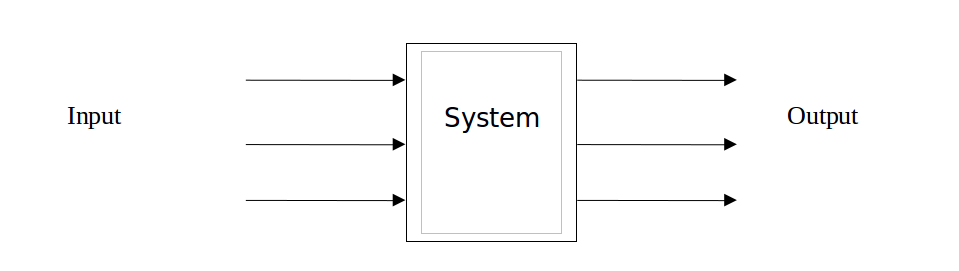
\includegraphics[scale=0.5]{images/LATEXREP001.png}
\end{center}
\caption{Functional Requirement}
\label{Functional Requirement}
\end{figure}



\section{Software Development Life Cycle Model}
\subsection{Spiral Model}
The spiral model is a risk-driven process model generator for software projects. Based on the
unique risk patterns of a given project, the spiral model guides a team to adopt elements of one
or more process models, such as incremental, waterfall, or evolutionary prototyping.

\begin{figure}[ht]
\begin{center}
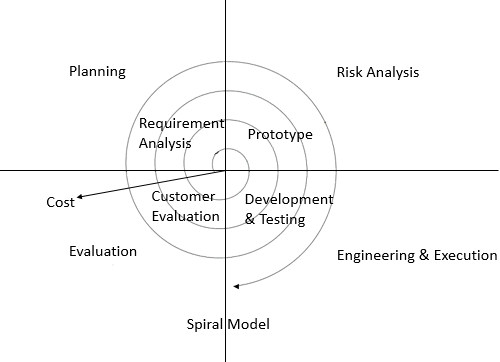
\includegraphics[scale=0.5]{images/spiralmodel.png}
\end{center}
\caption{Spiral Model}
\label{Spiral Model}
\end{figure}

\begin{itemize}
\item Planning Phase:\newline Requirements are gathered during the planning phase. Requirements like
BRS that is Bussiness Requirement Specifications and SRS that is System Requirement
specifications.
\item Risk Analysis: \newline
In the risk analysis phase, a process is undertaken to identify risk and alternate
solutions. A prototype is produced at the end of the risk analysis phase. If any risk is found
during the risk analysis then alternate solutions are suggested and implemented.
\item Engineering Phase: \newline
In this phase software is developed, along with testing at the end of the
phase. Hence in this phase the development and testing is done. Evaluation phase: This
phase allows the customer to evaluate the output of the project to date before the project
continues to the next spiral.
\end{itemize}



